% Options for packages loaded elsewhere
\PassOptionsToPackage{unicode}{hyperref}
\PassOptionsToPackage{hyphens}{url}
%
\documentclass[
]{article}
\usepackage{amsmath,amssymb}
\usepackage{iftex}
\ifPDFTeX
  \usepackage[T1]{fontenc}
  \usepackage[utf8]{inputenc}
  \usepackage{textcomp} % provide euro and other symbols
\else % if luatex or xetex
  \usepackage{unicode-math} % this also loads fontspec
  \defaultfontfeatures{Scale=MatchLowercase}
  \defaultfontfeatures[\rmfamily]{Ligatures=TeX,Scale=1}
\fi
\usepackage{lmodern}
\ifPDFTeX\else
  % xetex/luatex font selection
\fi
% Use upquote if available, for straight quotes in verbatim environments
\IfFileExists{upquote.sty}{\usepackage{upquote}}{}
\IfFileExists{microtype.sty}{% use microtype if available
  \usepackage[]{microtype}
  \UseMicrotypeSet[protrusion]{basicmath} % disable protrusion for tt fonts
}{}
\makeatletter
\@ifundefined{KOMAClassName}{% if non-KOMA class
  \IfFileExists{parskip.sty}{%
    \usepackage{parskip}
  }{% else
    \setlength{\parindent}{0pt}
    \setlength{\parskip}{6pt plus 2pt minus 1pt}}
}{% if KOMA class
  \KOMAoptions{parskip=half}}
\makeatother
\usepackage{xcolor}
\usepackage[top=5mm,bottom=20mm,left=10mm,right=10mm]{geometry}
\usepackage{graphicx}
\makeatletter
\def\maxwidth{\ifdim\Gin@nat@width>\linewidth\linewidth\else\Gin@nat@width\fi}
\def\maxheight{\ifdim\Gin@nat@height>\textheight\textheight\else\Gin@nat@height\fi}
\makeatother
% Scale images if necessary, so that they will not overflow the page
% margins by default, and it is still possible to overwrite the defaults
% using explicit options in \includegraphics[width, height, ...]{}
\setkeys{Gin}{width=\maxwidth,height=\maxheight,keepaspectratio}
% Set default figure placement to htbp
\makeatletter
\def\fps@figure{htbp}
\makeatother
\setlength{\emergencystretch}{3em} % prevent overfull lines
\providecommand{\tightlist}{%
  \setlength{\itemsep}{0pt}\setlength{\parskip}{0pt}}
\setcounter{secnumdepth}{-\maxdimen} % remove section numbering
\usepackage{hyperref}
\usepackage{graphicx}

\newcommand{\githublogo}{
  \noindent\href{https://github.com/ethraj2001/STAT447C_Bayesian_DVR_QPE}{
    
\includegraphics[scale=4]{tex/github.png}}
}


\usepackage{amsmath, amssymb, amsthm, tcolorbox}
\usepackage{geometry}
\usepackage{algorithm}
\usepackage{algpseudocode}
\usepackage{fancyhdr}
\usepackage{indentfirst}
\usepackage{multicol}
\usepackage{bbm}
\usepackage{dsfont}
\usepackage{physics}
\usepackage{titlesec}
\usepackage{float}
\usepackage{stfloats}
\usepackage{chemformula}
\usepackage{graphicx}
\usepackage[numbers, super]{natbib}
\usepackage{hyperref}
\usepackage{fancyhdr}
\usepackage{tikz}
\usepackage{wrapfig}
\usepackage{amsmath}
\usepackage{amssymb}
\usepackage{amsthm}
\usepackage{mdframed} % For creating the boxed environment
\newmdtheoremenv{definition}{Definition}
\usepackage{pdfpages}
\ifLuaTeX
  \usepackage{selnolig}  % disable illegal ligatures
\fi
\usepackage{bookmark}
\IfFileExists{xurl.sty}{\usepackage{xurl}}{} % add URL line breaks if available
\urlstyle{same}
\hypersetup{
  pdftitle={Estimation of Ro-Vibrational Eigenphases Using Bayesian Quantum Phase Estimation},
  hidelinks,
  pdfcreator={LaTeX via pandoc}}

\title{Estimation of Ro-Vibrational Eigenphases Using Bayesian Quantum
Phase Estimation}
\usepackage{etoolbox}
\makeatletter
\providecommand{\subtitle}[1]{% add subtitle to \maketitle
  \apptocmd{\@title}{\par {\large #1 \par}}{}{}
}
\makeatother
\subtitle{STAT 447C Final Project: Ethan Rajkumar, \#55024616}
\author{}
\date{\vspace{-2.5em}}

\begin{document}
\maketitle

\vspace{-1.5cm}
\maketitle
\begin{center}
\githublogo
\end{center}

\subsubsection*{\texorpdfstring{\underline{Introduction}}{}}\label{section}
\addcontentsline{toc}{subsubsection}{\underline{Introduction}}

\vspace{-0.5cm}

To analyze molecular characteristics, chemists often solve the following
eigenvalue equation: \begin{align}
    \mathbf{H}_{RV} \Psi(\vec{\theta}) &= E \Psi(\vec{\theta})
\end{align} In this equation, \(\mathbf{H}_{RV}\)represents the
Hamiltonian that accounts for the molecule's total ro-vibrational
energy. The wavefunction \(\Psi\), parameterized by the vector
\(\vec{\theta}\), serves as the eigenvector. The energy level \(E\)
corresponds to the eigenvalue which represents the energy levels
electrons can occupy. While simpler molecules like H\(_{2}\) allow for
straightforward single vector decompositions, larger molecules present
computational challenges due to the increased size of
\(\mathbf{H}_{RV}\). This project aims to address these challenges by
using quantum phase estimation to estimate a posterior distribution,
which can then be used to estimate the eigenvalues of
\(\mathbf{H}_{RV}\) for the Cr\(_2\) molecule. \vspace{-0.5cm}

\subsubsection*{\texorpdfstring{\underline{Literature Review}}{}}\label{section-1}
\addcontentsline{toc}{subsubsection}{\underline{Literature Review}}

\vspace{-0.5cm}

Taking the ro-vibrational Hamiltonian \(\mathbf{H}_{RV}\) and performing
the following operation to form a matrix \(\mathcal{U}\) gives
\(\mathcal{U} = e^{i \mathbf{H}_{RV} t}\). The expression above allows
for the application of the phase estimation algorithm, which estimates
the eigenvalues of the unitary operators. The algorithm then uses these
eigenvalues to approximate the eigenvalues of the original Hamiltonian.
A matrix is denoted to be unitary if it follows the spectral theorem
which is listed below. \vspace{-0.1cm}

\begin{mdframed}
\textbf{Spectral Theorem:}
Let \( U \) be a normalized \( K \times K \) complex matrix. There exists an orthonormal basis of \( K \)-dimensional complex vectors \( \{|\psi_1\rangle, \dots, |\psi_K\rangle\} \), along with complex numbers \( \lambda_1, \dots, \lambda_K \), such that 
\( U = \lambda_1 |\psi_1\rangle \langle \psi_1| + \cdots + \lambda_K |\psi_K\rangle \langle \psi_K|.\)
This matrix \( U \) can be diagonalized in an orthonormal basis consisting of its eigenvectors, with the corresponding eigenvalues on the diagonal.
\end{mdframed}
\vspace{-0.1cm}

The main implementation of the phase estimation algorithm is shown
below:

\begin{mdframed}
\textbf{Quantum Phase Estimation Algorithm:}
\begin{itemize}
\item \textbf{Input:}
An \( n \)-qubit quantum state \( |\psi\rangle \) and a unitary quantum circuit for an \( n \)-qubit operation \( U \).
\item \textbf{Promise/Assumptions:}
\( |\psi\rangle \) is an eigenvector of \( U \).
\item \textbf{Output:}
An approximation to the number \( \theta \in [0,1) \) satisfying 
\(U |\psi\rangle = e^{2\pi i \theta} |\psi\rangle.\)
\end{itemize}
\end{mdframed}

Quantum phase estimation can also take a probabilistic approach in the
form of Bayesian optimization. Termed Bayesian Quantum Phase Estimation
by Weibe and Granade in 2016 \cite{Weibe2016}. It was made efficient in
a highly noisy environment by Yamamoto et al.~(2024)
\cite{Yamamoto2023}. This method uses a quantum circuit to represent the
posterior distribution of the phase estimation algorithm
\cite{Weibe2016, Yamamoto2023}. For a two-qubit circuit, the authors
used a quantum circuit which is an acyclic network of quantum gates
connected by wires. The quantum gates are matrices that represent
quantum operations while the wires represent the \textbf{qubits} (see
appendix) on which the gates act. The pictorial representation of the
circuit is shown in Figure 1 (below).

\begin{wrapfigure}{r}{0.40\textwidth}
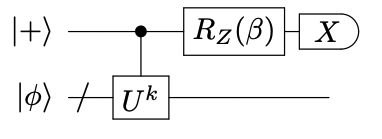
\includegraphics[width=0.40\textwidth]{tex/circuit.png}
\end{wrapfigure}

The quantum circuit is parameterized by \(k \in \mathbb{N}\) and
\(\beta \in [0 , 1]\). The circuit is measured in the Pauli X basis and
the measurement is denoted as a probability of states (or a likelihood)
in the computational basis such that
\(p(m\vert \phi, k, \beta) = \frac{1 + \cos(k\phi + \beta)}{2}\) where
\(m\) is the measurement outcome in the computational basis, \(\phi\) is
the unknown where \(p(\phi)\sim \text{Unif}[0, 2\pi)\), and RZ is a
rotational matrix described in the appendix below. With \(R\) possible
measurement outcomes and a high number of iterations, a posterior
distribution can be computed such that
\(p(\phi \vert m, k, \beta) \propto p(\phi) \cdot \Pi^R_{r=1}p_{r}(m\vert \phi, k, \beta)\).
Once converged, the probability distributions are then used to compute a
posterior mean with respect to an observable or
\(\sum_R p(\phi \vert m, k, \beta) \langle  R | \hat{H} | R \rangle\).
Note that this work does not compute a posterior mean but instead
creates the probabilities that will estimate the eigenvalues of the
Hamiltonian matrix. \vspace{-0.7cm}

\subsubsection*{\texorpdfstring{\underline{Problem Formulation}}{}}\label{section-2}
\addcontentsline{toc}{subsubsection}{\underline{Problem Formulation}}

\begin{wrapfigure}{r}{0.40\textwidth}
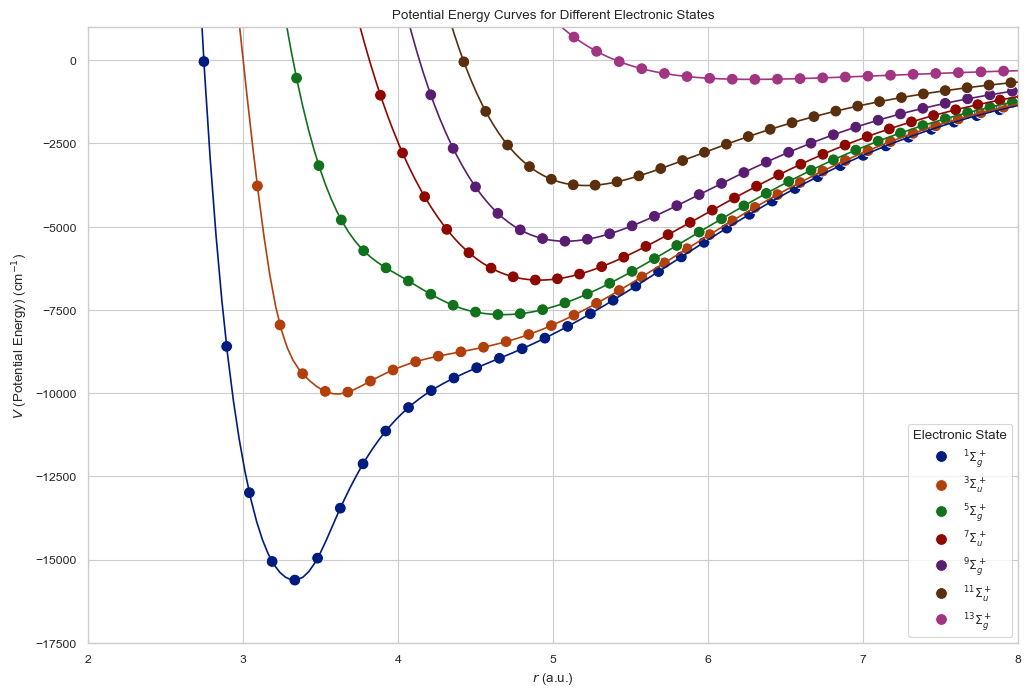
\includegraphics[width=0.40\textwidth]{tex/potentialenergygraph.png}
\end{wrapfigure}

While Asnaashari et al.~employed a hybrid quantum-classical computing
approach to address an eigenvalue problem, using a greedy induced point
sampling algorithm to compute an expectation in their respective basis,
they encountered significant scalability issues related to the time
complexity of quantum circuit generation, denoted by
\(\mathcal{O}(\sum_k n \times M_k )\), where \(M_k\) represents the time
required to generate an expectation value per iteration over \(n\)
samples, and \(k\) denotes the iteration index
\cite{asnaashari2023compact}. Yamamoto and Weibe attempted to use
quantum phase estimation of a different type of Hamiltonian to compute
the eigenphase/eigenvalues in the computational basis
\cite{Yamamoto2023, Weibe2016}. However, their method only uses up to 2
qubits, required 920 gates and is not scalable to a higher amount of
qubits. The key challenge that this project aims to address is to create
an algorithm that has a minimum of 5 qubits while also having a lower
gate count (12) while also being accurate. The project algorithm, which
is based on the Bayesian Quantum Phase Estimation algorithm, will be
used to estimate the eigenvalues of the Hamiltonian matrix for the
dichromium molecule. Further literature review showed that very few
papers have been published on the topic and that the Bayesian Quantum
Phase Estimation algorithm has not been used to estimate the eigenvalues
of the Hamiltonian matrix for the Cr\(_2\) molecule.

\vspace{-0.5cm}

\subsubsection*{\texorpdfstring{\underline{Data Preprocessing and Generation of Unitary Matrices}}{}}\label{section-3}
\addcontentsline{toc}{subsubsection}{\underline{Data Preprocessing and Generation of Unitary Matrices}}

\vspace{-0.5cm}

The data used in this project was generated by Asnaashari and is a
discrete variable representation of the Hamiltonian
\cite{asnaashari2023compact}. First, an interpotential curve (measures
the Coulombic interaction of two atoms) was generated from Fortran for
the Cr\(_2\) molecule (graph on the right). Afterwards, a Hamiltonian
matrix was selected from the 32 points collected from the curve for each
spin state. A combination of the \texttt{pennylane} and \texttt{phayes}
Python 3.11.7 libraries were used to transform the Hamiltonian matrix
into a unitary matrix as described in the literature review. The unitary
matrix was then used to generate the quantum circuit by applying a
transform: \begin{align}
    U = e^{i \mathbf{H}_{RV} t} 
\end{align} The quantum circuit was then used to estimate the phases,
\(\phi\), of each unitary matrix. The phase estimation algorithm itself
can be described by the probabilistic model below. \vspace{-0.5cm}

\subsection*{\texorpdfstring{\underline{Model}}{}}\label{section-4}
\addcontentsline{toc}{subsection}{\underline{Model}}

\vspace{-0.5cm}

The model used in this project is a Bayesian model that estimates the
phases of the unitary matrices. The model is parameterized by the number
of qubits, \(n\), and the number of iterations, \(R\). The model is
defined as follows (using the \(\sim\) notation): \vspace{-0.2cm}
\begin{align*}
   \mathcal{L} &= (m | \phi,  \beta, k)  \sim \text{Fourier Distribution{\beta}} \\
   \phi &\sim \text{Unif}(0, 2\pi) \\
   \beta &\sim \text{Unif}(0, 2\pi) \\ 
    k &\sim \mathcal{N}(\alpha, \sqrt{1/\sigma^2}) \\  
    \alpha &\sim \text{Unif}[J, J_{max}] \text{ where \(J\) and \(J_{max}\)} \in \mathbb{N}
\end{align*}

\vspace{-0.2cm}

The quantum circuit provided in the literature review is used to
estimate the phases of the unitary matrices. Note that we are trying to
estimate \(\phi\) and the error compared to the true value, \(\phi_{0}\)
which is the angle(s) or phase that we are trying to estimate. The error
is denoted as \(\epsilon = \phi - \phi_0\). The error is then used to
estimate the eigenvalues of the Hamiltonian matrix. Note that the phases
will be estimated for multiple spin states of dichromium gas. The
likelihood and prior are defined below:

\vspace{-0.2cm}

\begin{mdframed}
\begin{itemize} 
\item \textbf{Likelihood}: This is defined by the quantum circuit as given by the first figure above. It is parameterized with \(k \in \mathbb{N}\) and \(\beta \in [0, 2\pi)\).  
\begin{align*}
    \mathbb{P}(m \vert \phi, k, \beta) &= \frac{1 + \cos(k\phi + \beta)}{2}  \text{ decomposition into the product form gives,}\\ 
    \mathbb{P}(m \vert \phi, k, \beta) &= \Pi^R_{r=1} p(m_r \vert \phi, k, \beta)
\end{align*}
\item \textbf{Prior} This is the probability of phi or equivalently $\mathbb{\phi}$ 
\begin{align*}
    \mathbb{P}(\phi) &\sim \text{Unif}[0, 2\pi)
\end{align*}
\end{itemize}
\end{mdframed}

\vspace{-0.2cm}

Thus the posterior that is being is estimated is described by:
\vspace{-0.2cm} \begin{align*}
     \mathbb{P}(\phi \vert m, k, \beta) \propto \mathbb{P}(\phi) \cdot \Pi^R_{r=1} \mathbb{P}(m_r \vert \phi, k, \beta)
\end{align*} \vspace{-0.1cm} The posterior is then used to estimate the
angle or phase of the unitary matrix by computation of a posterior mean
for the phase. The evaluation metric used for this model is
\(\epsilon =  \vert \phi - \phi_{0} \vert\). This particular error
metric is used as the model and the true phases are evaluated in the
same basis for each spin state.

\subsection*{\texorpdfstring{\underline{Results}}{}}\label{section-5}
\addcontentsline{toc}{subsection}{\underline{Results}}

The graph below shows the \(\epsilon\) values for each of the unitary
matrices for all of the spin states. The errors was obtained by taking
the synthetic unitary data (100 experiments) and subtracting the true
value (for each eigenvalue) from the result. Afterwards, each result was
graphed on a cubic spline with an offset of 0.04 radians. This is so the
results for all of the spin states can be easily visualized.

\begin{figure}[H]
\centering
\caption{Phase Error For Each Spin State (with respect to the Index of the Eigenphase)}
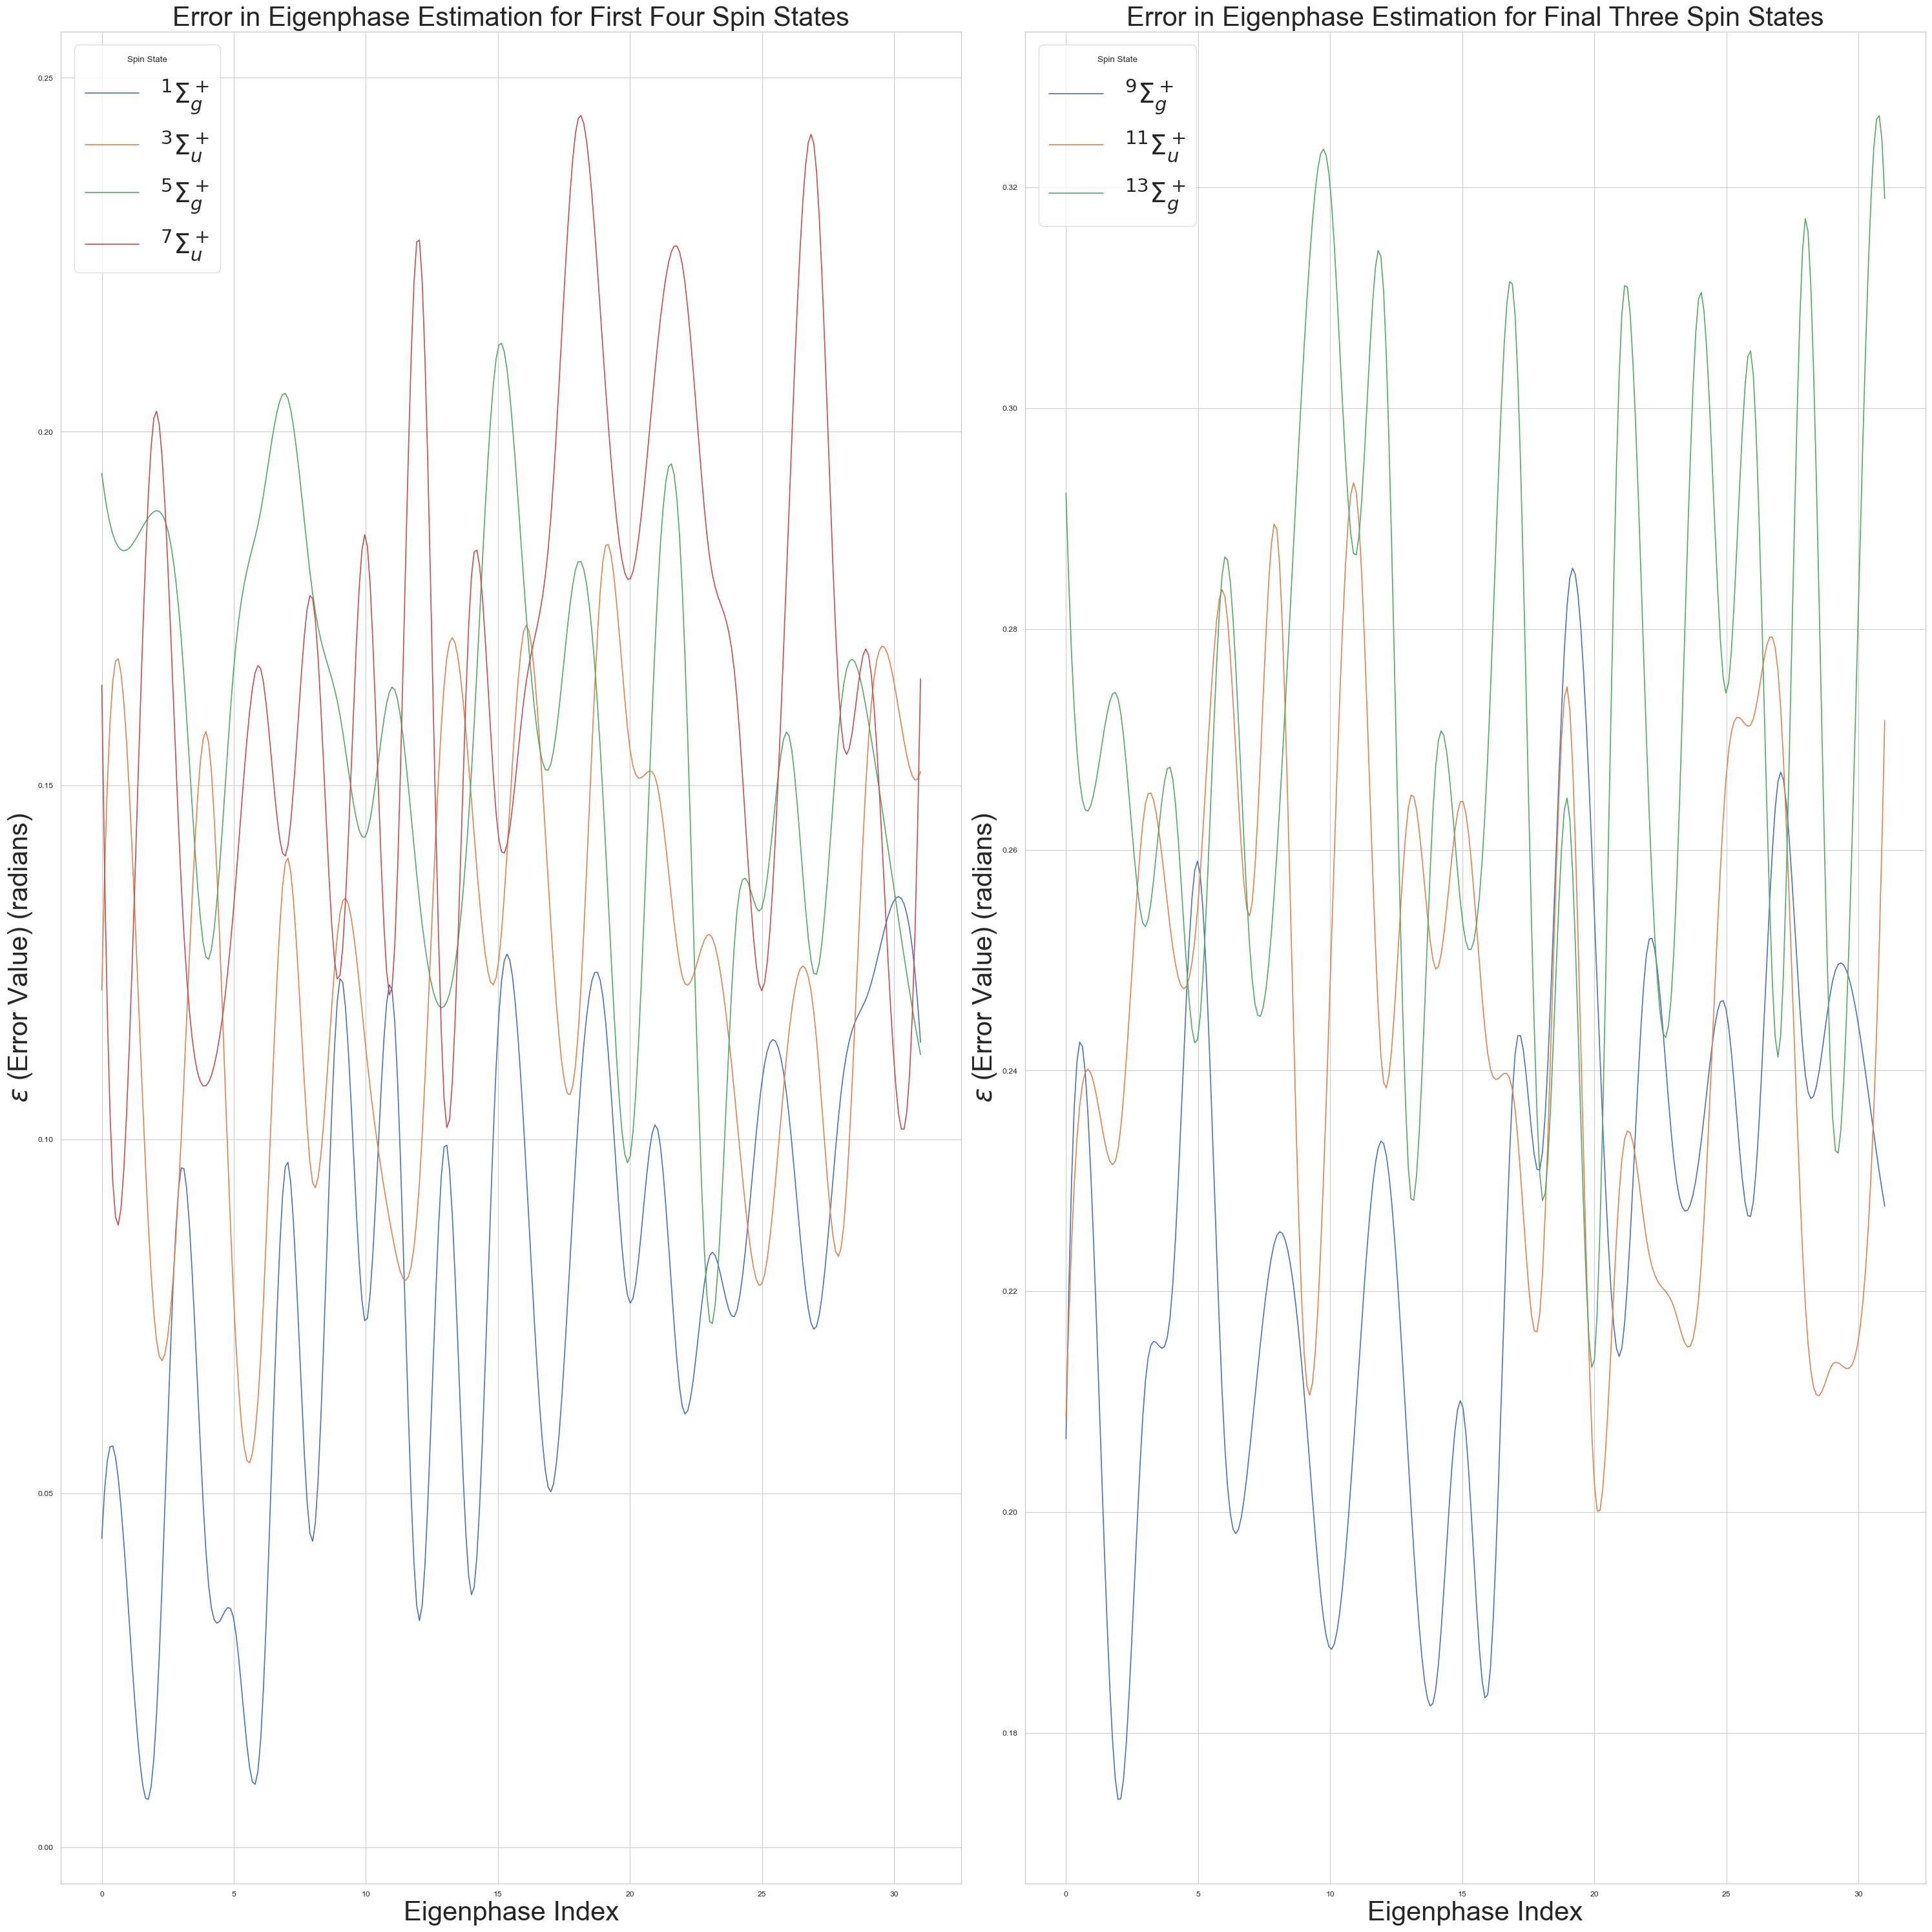
\includegraphics[width=0.6\textwidth]{tex/2D_graph.png}
\end{figure}

The graph indicates that error rates are somewhat low for the 2D graph.
The error manifests a sinusoidal pattern with respect to the eigenphase
index, which is not uniform across the various spin states.
Specifically, the error for the initial spin state
(\({}^1\Sigma_{g}^+\)) averages significantly lower in comparison to
that of the subsequent spin states. There is a notable increase in error
when progressing from the first to the second spin state. The seventh
and thirteenth spin states exhibit the most pronounced errors, which
coincide with the greatest fluctuations in the variable \(\epsilon\). To
determine the extent to which k and \(\beta\) values affect the error,
3D graphs were created to show the relationship between the error and
the k and \(\beta\) values.

\begin{figure}[H]
\centering
\caption{Phase Error For Each Spin State}
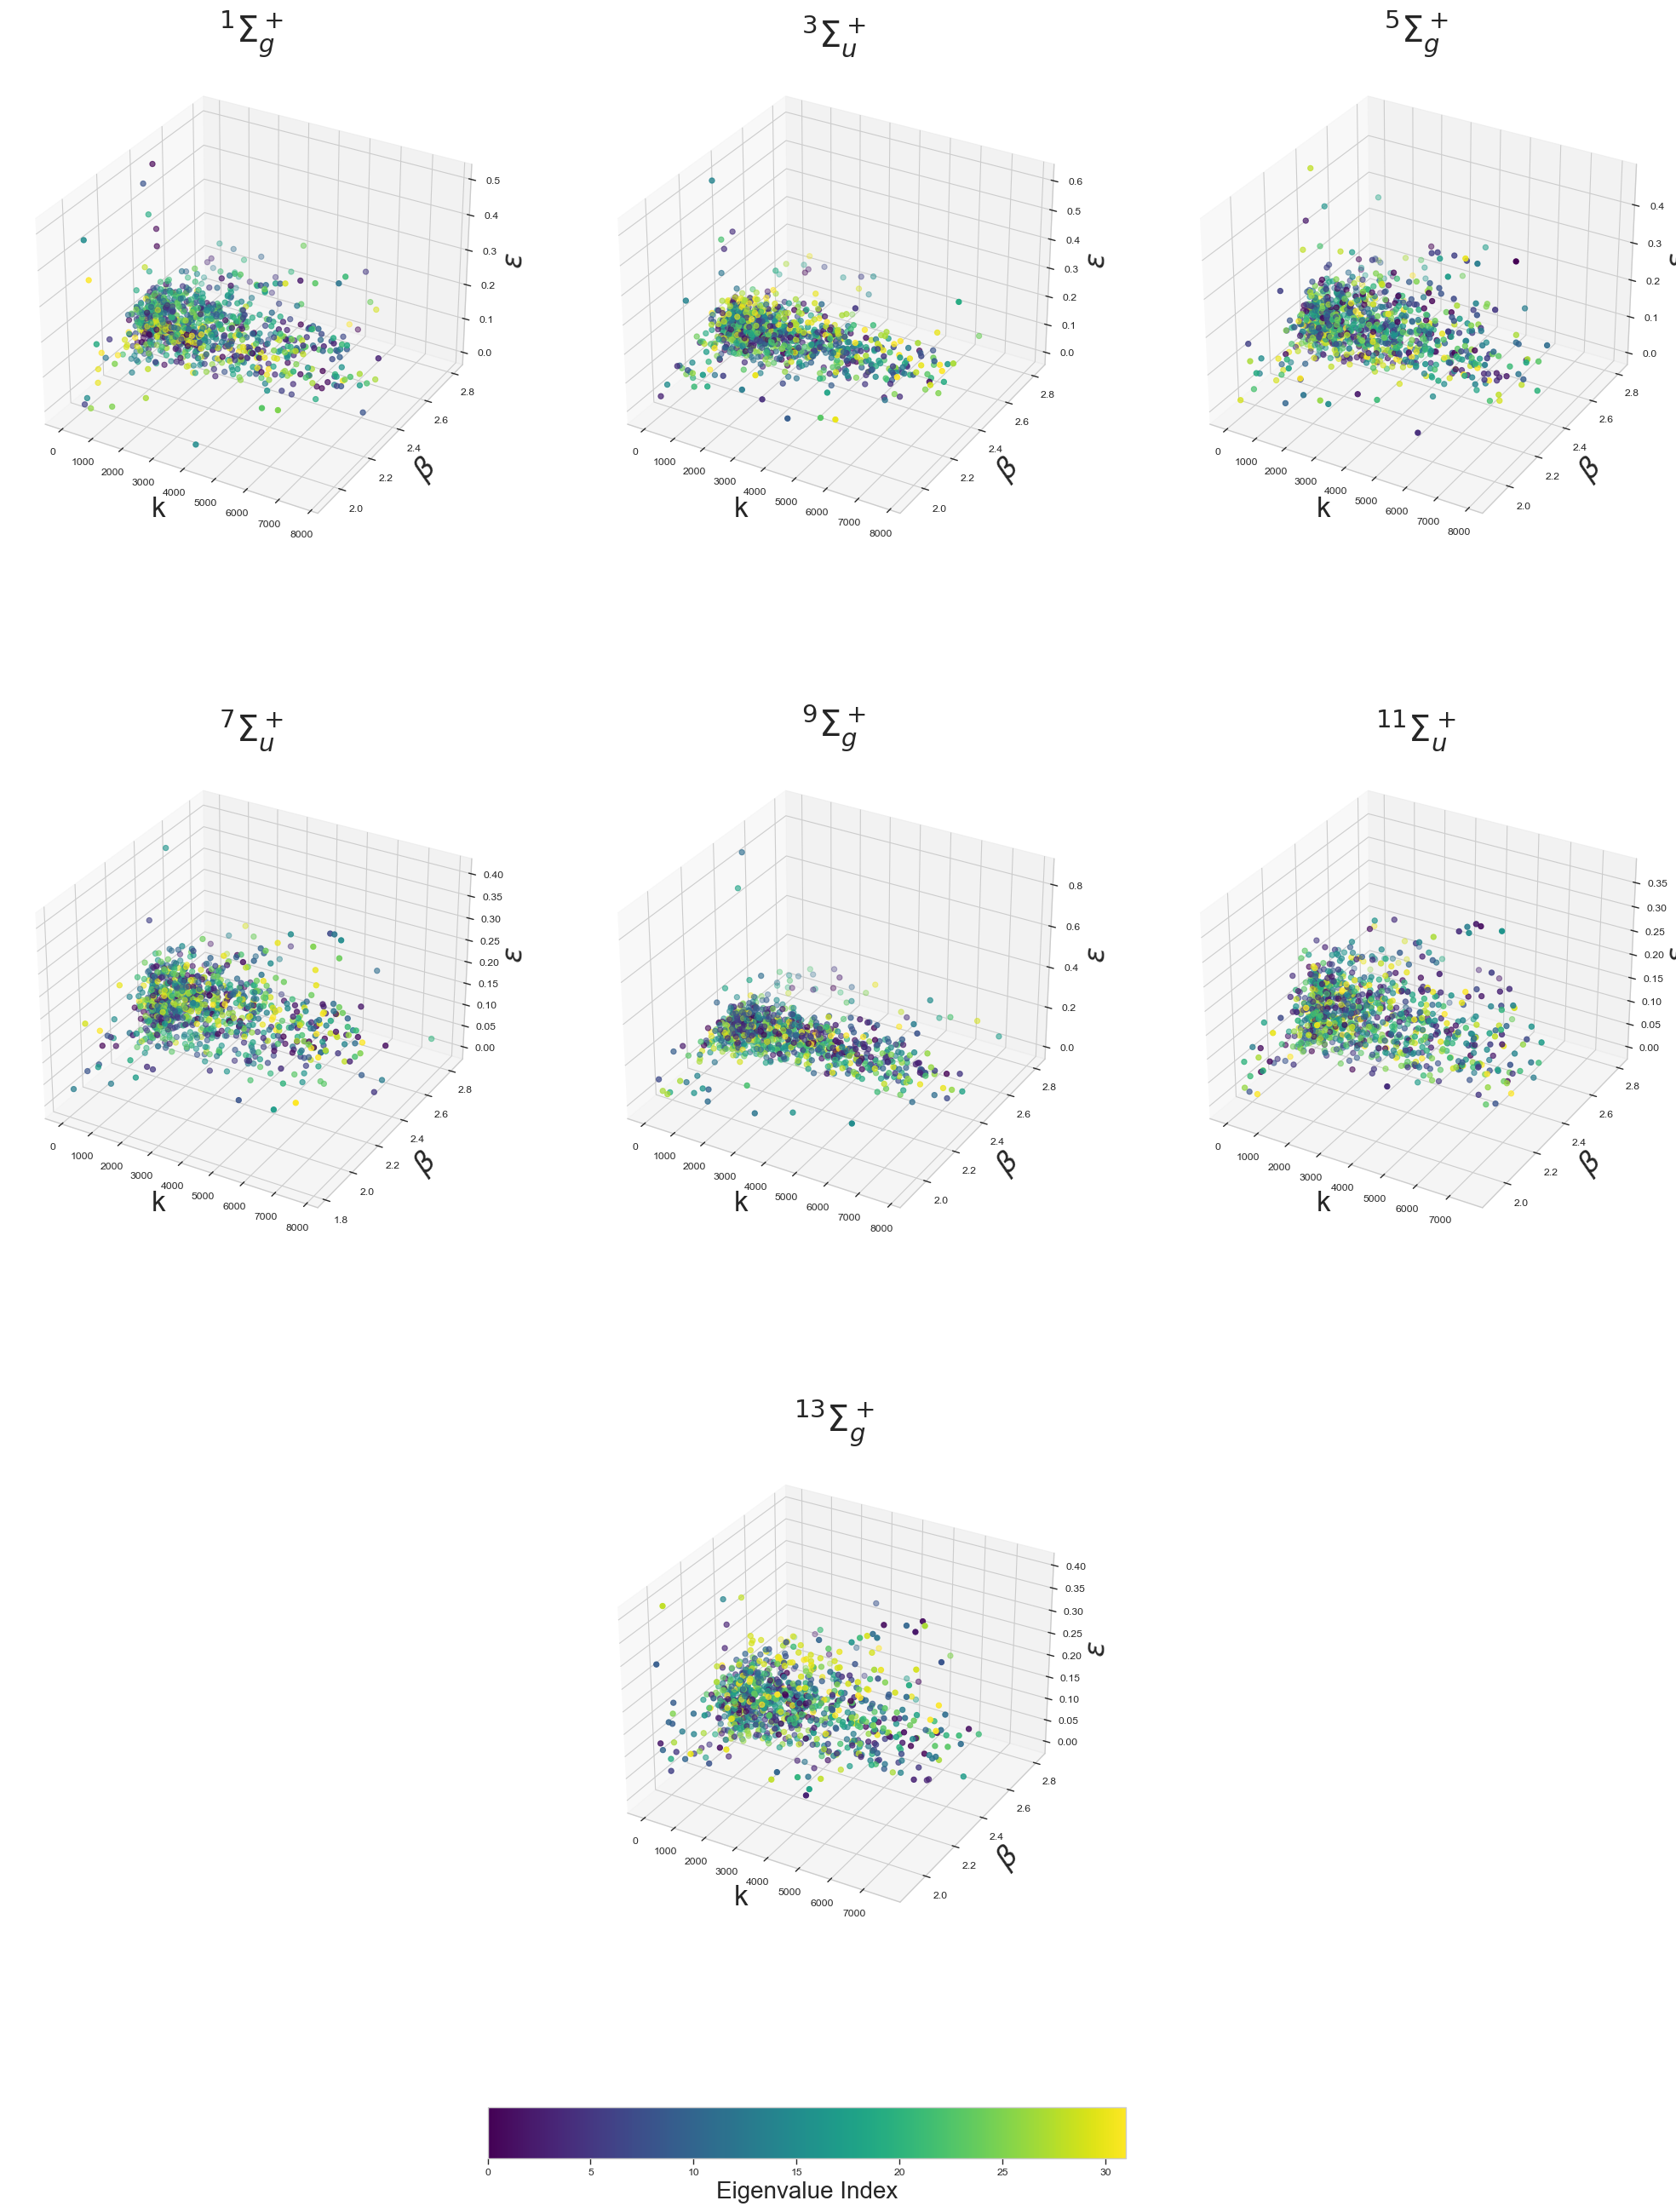
\includegraphics[width=0.6\textwidth]{tex/3D_graph.png}
\end{figure}

The 3D plots show a pronounced clustering of data points within specific
areas for all states, indicative of a localized aggregation of
eigenvalues and possibly contributing to the consistently lower and more
predictable error rates for this state. The compactness of these
clusters suggests stability in the eigenvalues relative to changes in
the parameters \(k\) and \(\beta\). Conversely, the \(7^1\Sigma_u^+\)
and \(13^1\Sigma_g^+\) states demonstrate a wider spread of data points
across the 3D space. This greater spread could be symptomatic of higher
and more variable error rates, hinting at less stability or precision in
these states. The scattered distribution points to a more pronounced
variation in eigenvalues in response to \(k\) and \(\beta\).
Additionally, the significant overlap of data at elevated \(k\) and
\(\beta\) values suggests a closeness or even degeneracy in the
eigenvalues, further compounding the variability of errors observed.
However the graph above suggests that model misspecification is highly
unlikely as the error rates are relatively low and the model is robust
to the assumptions it holds. The error with respect to the
hyperparameters \(k\) and \(\beta\) (for all eigenvalues) occupys a
approximately normal distribution indicating that it can be improved by
adding a constant to the phase estimation.

Finally, a posterior distribution was obtained to determine the
distributions of the phases given the hyperparameters, \(k\) and
\(\beta\).

\begin{figure}[H]
\centering
\caption{Posterior Distribution For Each Spin State}
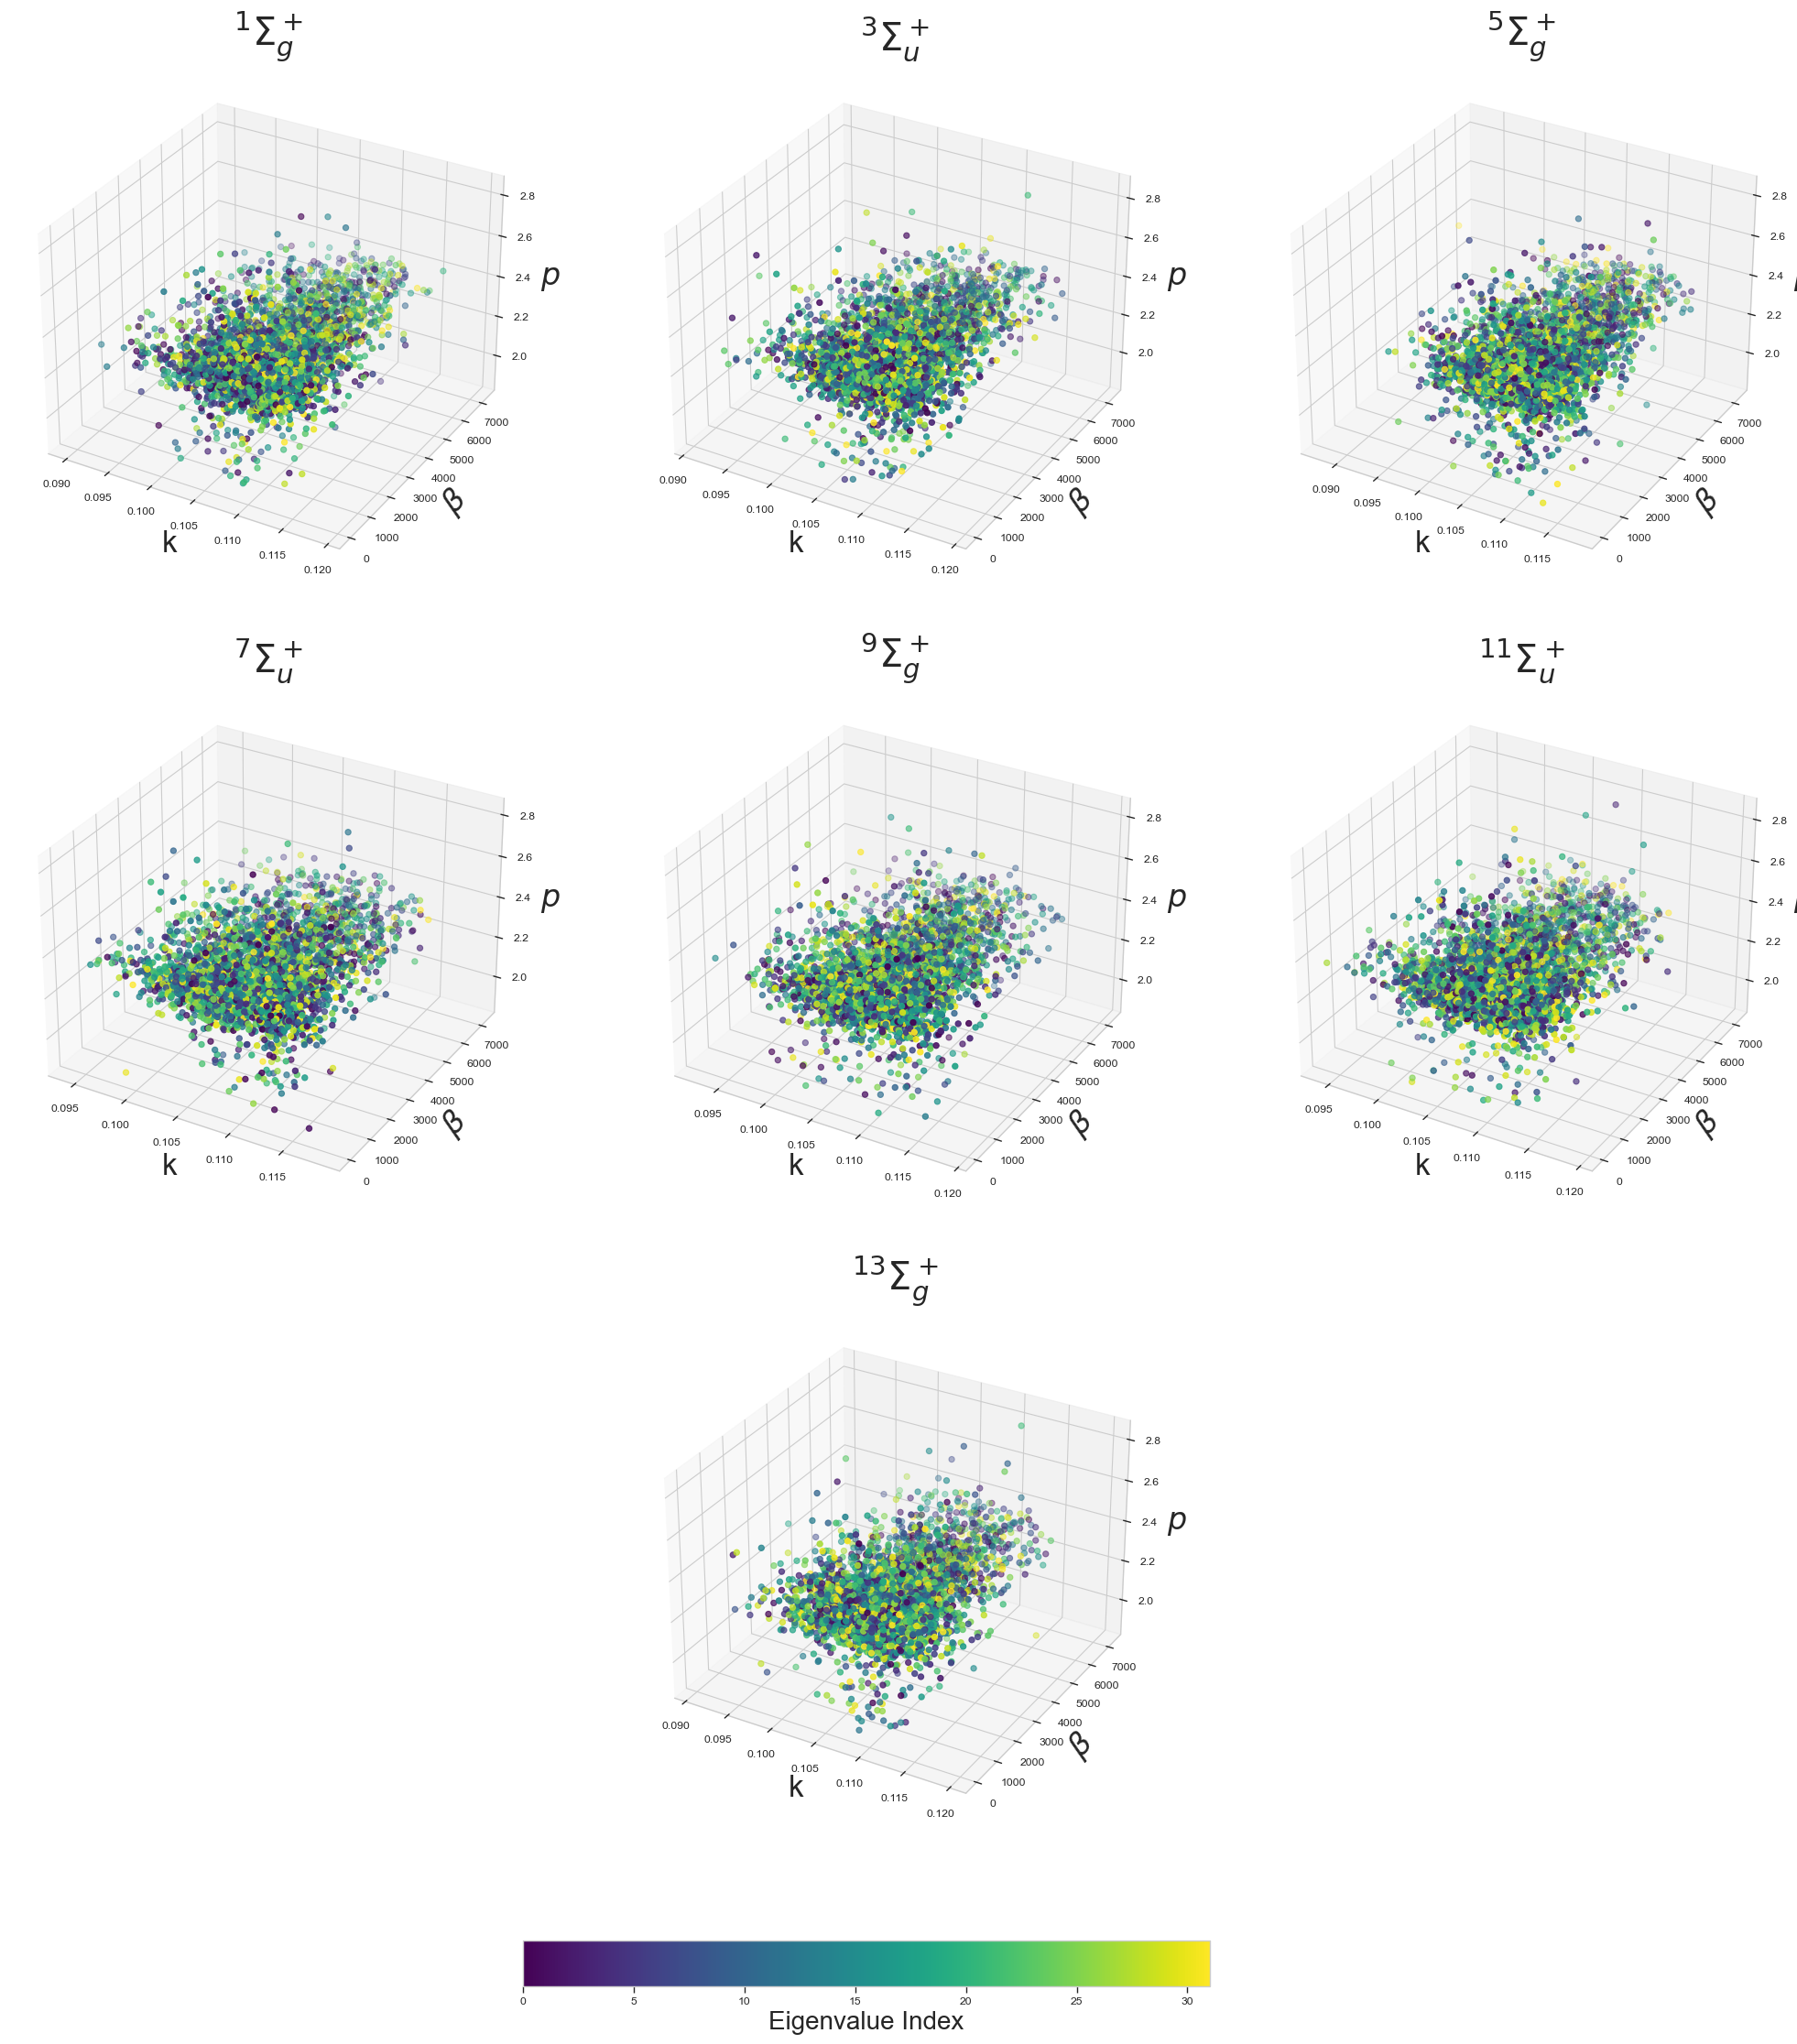
\includegraphics[width=0.6\textwidth]{tex/posteriorgraph.png}
\end{figure}

The posterior can be described as an approximately slanted round sheet
clustered.The tight clustering of points within the graph suggests a
higher certainty about the phase \(\phi\) for the corresponding
eigenvalue index, whereas a wider spread of points is indicative of
greater uncertainty. When correlated with the results from the 3D phase
error graph, it is suggested that lower \(k\) values and lower \(\beta\)
are associated with higher conditional probabilities of a phase and a
greater phase error when compared to the true phase value. A sensitivity
analysis could not be performed as the true distribution of the phases
is unknown.

\subsection*{\texorpdfstring{\underline{Discussion}}{}}\label{section-6}
\addcontentsline{toc}{subsection}{\underline{Discussion}}

The results of this study demonstrate that the extrapolation behavior of
the model is proficient at determining the phases for a dichromium
molecule, with a low error rate observed. The posterior distribution
tends to follow a normal distribution across all eigenvalues and
eigenvectors, in relation to the hyperparameters \(k\) and \(\beta\).
Consequently, these phases can be transformed to estimate the
eigenvalues of the Hamiltonian, which in turn correspond to the discrete
energy levels accessible to electrons.

However, the model is subject to certain limitations. Its stochastic
nature, particularly when it is assumed to be time-independent,
introduces variability that can lead to different simulation outcomes
despite identical initial conditions, complicating the reproducibility
of results and precise behavior prediction. Additionally, as the size of
the molecule increases, the assumptions integral to the stochastic model
may not remain valid across all scenarios. The inherent randomness of
\(k\) and \(\beta\) may not accurately reflect the molecule's actual
physical attributes, leading to possible model misspecification.
Computational issues, such as underflow, present further challenges; as
the molecular size escalates, the number of computational basis states
expands exponentially. This is predicated on the assumption that the
molecule may only uniformly occupy each state, which could amplify the
model's sensitivity to initial conditions. Lastly, inherent to the
definition of stochastic models is the potential oversight of quantum
entanglement (the superposition of states)---an essential aspect of
quantum mechanics that, if not accurately represented, could induce
significant errors in the modeling of the posterior of \(\phi\)
\cite{Yamamoto2023}.

\subsection*{\texorpdfstring{\underline{Conclusion and Future Directions}}{}}\label{section-7}
\addcontentsline{toc}{subsection}{\underline{Conclusion and Future Directions}}

Despite these limitations, the model does offer a flexible and
interpretable approach to Quantum Phase Estimation. By showing a high
degree of accuracy for \(\phi\), the model can be used to estimate the
eigenvalues of the Hamiltonian matrix for the Cr\(_2\) molecule. Future
work could focus on improving the model's scalability and robustness to
larger molecules such as ArHCl. This could involve the development of a
more efficient quantum circuit that can handle a higher number of
qubits, as well as the implementation of a more sophisticated Bayesian
optimization algorithm to improve the model's accuracy and precision.
Additionally, the model could be extended to include more complex
quantum operations and gates, enhancing its capabilities and
applicability to a wider range of molecular systems. Finally the model
could be used in other applications than chemistry such as electronics
engineering (phases for batteries).

By addressing these challenges and limitations, the model could become a
valuable tool for chemists, physicists and engineering seeking to
analyze the ro-vibrational properties of complex molecules and
materials.

\bibliographystyle{achemso}
\bibliography{tex/manuscript.bib}

\subsection*{Acknowledgements}\label{acknowledgements}
\addcontentsline{toc}{subsection}{Acknowledgements}

I would like to thank Professor Roman Krems and Kasra Asnaashari for the
data used, their guidance and support throughout this project. I would
also like to thank the University of British Columbia for providing the
resources necessary to complete this project.

\subsection*{\texorpdfstring{\underline{Appendix}}{}}\label{section-8}
\addcontentsline{toc}{subsection}{\underline{Appendix}}

\subsubsection*{\texorpdfstring{\underline{A: Glossary of Some Quantum Computing Terms}}{}}\label{section-9}
\addcontentsline{toc}{subsubsection}{\underline{A: Glossary of Some Quantum Computing Terms}}

\paragraph*{\texorpdfstring{\underline{Bra}}{}}\label{section-10}
\addcontentsline{toc}{paragraph}{\underline{Bra}}

A row vector defined by:

\begin{align}
   \langle  \psi \vert = \big [ \psi^\dagger_{1}, \psi^\dagger_{2}, ... , \psi^\dagger_{K} \big]
\end{align}

where \(\psi^\dagger\) is the complex conjugate of \(\psi\).

\paragraph*{\texorpdfstring{\underline{Ket}}{}}\label{section-11}
\addcontentsline{toc}{paragraph}{\underline{Ket}}

A column vector defined by: \begin{align*}
    \vert \psi \rangle  = \big [ \psi_{1}, \psi_{2}, ... , \psi_K \big]^T
\end{align*}

\paragraph*{\texorpdfstring{\underline{Qubit}}{}}\label{section-12}
\addcontentsline{toc}{paragraph}{\underline{Qubit}}

Represented by a complex-valued, \(2 \times 1\) vector. It can be
written as a linear combination of \(\ket{0}\) and \(\ket{1}\) as
follows: \[
\ket{\psi} = \alpha\ket{0} + \beta\ket{1}
\] where \(\alpha\) and \(\beta\) are complex numbers, and
\(|\alpha|^2 + |\beta|^2 = 1\). Note that \begin{align}
    \vert 0 \rangle  &=  [1 , 0]^T ,  \vert 1 \rangle = [0, 1]^T 
\end{align}

One does not observe \(\alpha\) and \(\beta\). Instead \(|\alpha|^2\)
and \(|\beta|^2\) are the coefficients that we observe. Each of
\(|\alpha|^2\) and \(|\beta|^2\) and beta correspond to the probability
of collapsing to a specific state.

\paragraph*{\texorpdfstring{\underline{Computational Basis States}}{}}\label{section-13}
\addcontentsline{toc}{paragraph}{\underline{Computational Basis States}}

Refers to the standard orthonormal basis for the state space of \(n\)
qubits and represents a complete set of orthonormal vectors for this
space. For a single qubit, the computational basis consists of the two
states \(\ket{0}\) and \(\ket{1}\). Each computational basis state for a
system of \(n\) qubits can be described as a tensor product of \(n\)
single-qubit states, where each qubit is independently in either
\(\ket{0}\) or \(\ket{1}\). The computational basis states form an
orthonormal basis, which implies that they are mutually orthogonal and
each has unit norm. The completeness of this basis set means that any
state \(\ket{\psi}\) of the system can be uniquely expressed as a linear
combination of these basis states, and no other states need to be added
to fully describe the state space. Each basis state corresponds to a
unique binary string of length \(n\), which is particularly useful for
encoding and manipulating information in quantum computation. The
general form of a computational basis state for an \(n\)-qubit system
is:

\[
\ket{i_{1} i_{2} \dots i_{n}} = \ket{i_{1}} \otimes \ket{i_{2}} \otimes \cdots \otimes \ket{i_{n}}
\]

where \(i_k\) is either 0 or 1, representing the state of the \(k\)-th
qubit. For example, in a two-qubit system, the computational basis
states are \(\ket{00}\), \(\ket{01}\), \(\ket{10}\), and \(\ket{11}\),
corresponding to the vector representations \([1, 0, 0, 0]^T\),
\([0, 1, 0, 0]^T\), \([0, 0, 1, 0]^T\), and \([0, 0, 0, 1]^T\)
respectively. Note that \(\ket{00} = \ket{1}\) , \(\ket{01}= \ket{2}\),
\(\ket{10}= \ket{3}\), and \(\ket{11}=\ket{4}\). This is because the
number of computational basis states \((k)\) is proportional to the
number of qubits \((N)\) such that

\begin{align}
k = 2^N  
\end{align}

\paragraph*{\texorpdfstring{\underline{Hardware Basis States}}{}}\label{section-14}
\addcontentsline{toc}{paragraph}{\underline{Hardware Basis States}}

Refers to the set of gates or operations that a quantum computer can
physically interpret and execute. The hardware basis

\subsubsection*{\texorpdfstring{\underline{B: List of Quantum Gates Used in this Work}}{}}\label{section-15}
\addcontentsline{toc}{subsubsection}{\underline{B: List of Quantum Gates Used in this Work}}

\paragraph*{\texorpdfstring{\underline{Pauli-Z Gate (\(Z\))}}{}}\label{section-16}
\addcontentsline{toc}{paragraph}{\underline{Pauli-Z Gate (\(Z\))}}

\[
  Z = \begin{bmatrix}
  1 & 0 \\
  0 & -1
  \end{bmatrix}
  \]

\paragraph*{\texorpdfstring{\underline{RZ Gate}}{}}\label{section-17}
\addcontentsline{toc}{paragraph}{\underline{RZ Gate}}

\[
  R_{z,x_k}\left(\theta \right) = \begin{bmatrix}
  e^{-i\theta \cdot x_k} & 0 \\
  0 & e^{i\theta \cdot x_k} 
  \end{bmatrix}
  \]

\includepages[pages=-]{tex/appendix_c.pdf}

\end{document}
